\documentclass{standalone}
\usepackage{tikz}
\usetikzlibrary{patterns}
\usetikzlibrary{positioning}
\usetikzlibrary{patterns, positioning}
\usetikzlibrary{shapes.misc}
\usepackage[outline]{contour}
\contourlength{1.5pt} 
\usepackage[sfdefault]{ClearSans}

\begin{document}
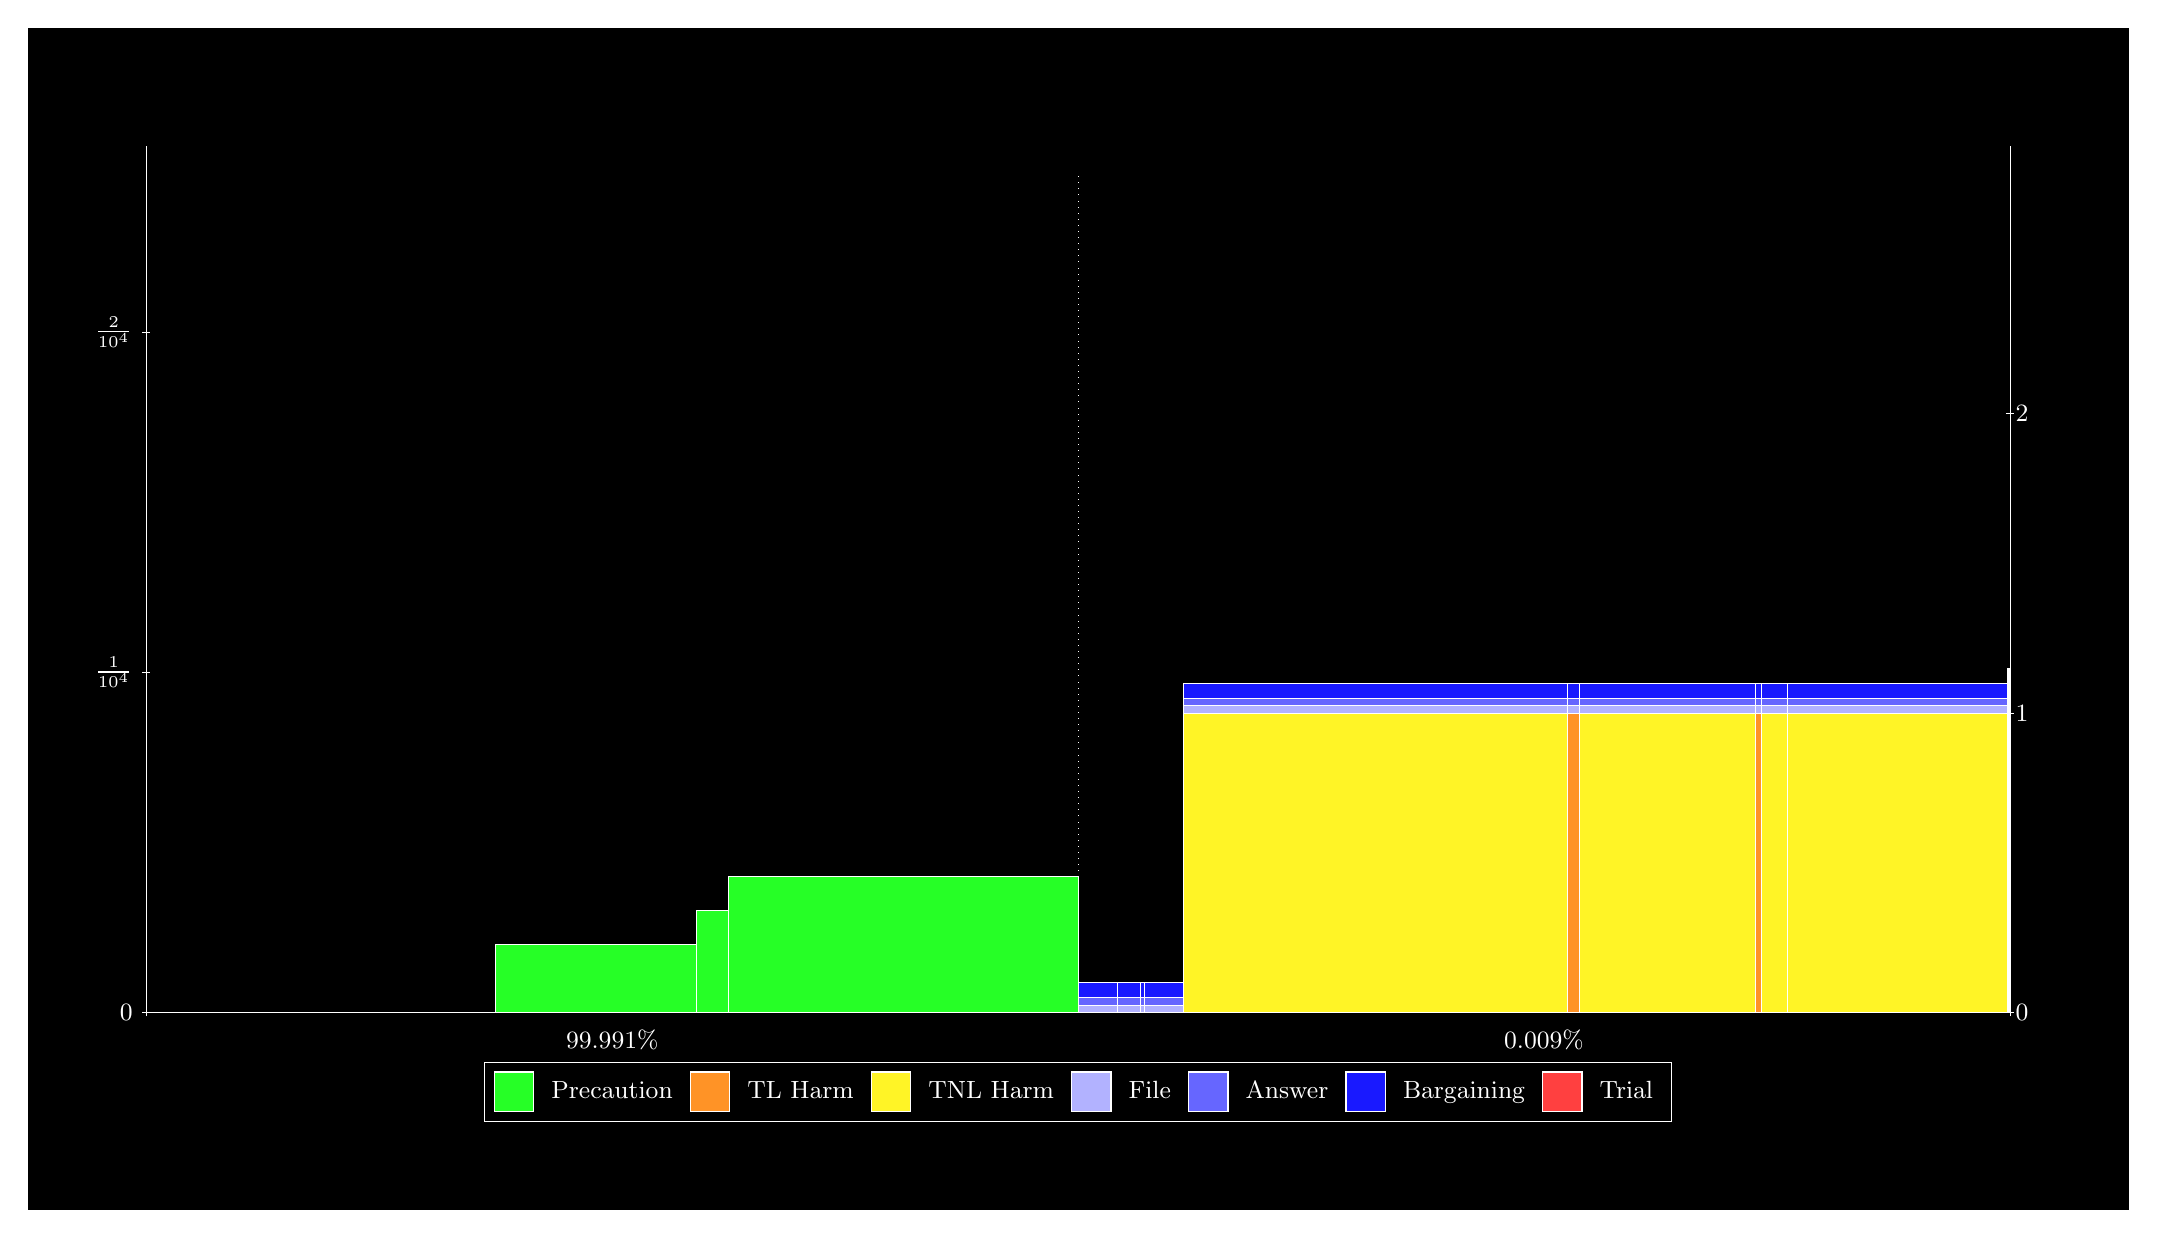
\begin{tikzpicture}
\draw[fill=black] (0,0) rectangle (26.667,15);
\draw[fill=green!85,draw=white,very thin] (5.9374,2.5) rectangle (8.4789,3.3641);
\draw[fill=green!85,draw=white,very thin] (8.4789,2.5) rectangle (8.8957,3.7962);
\draw[fill=green!85,draw=white,very thin] (8.8957,2.5) rectangle (13.333,4.2282);
\draw[fill=blue!30,draw=white,very thin] (13.333,2.5) rectangle (13.836,2.595);
\draw[fill=blue!60,draw=white,very thin] (13.333,2.595) rectangle (13.836,2.6901);
\draw[fill=blue!90,draw=white,very thin] (13.333,2.6901) rectangle (13.836,2.8802);
\draw[fill=green!85,draw=white,very thin] (13.836,2.5) rectangle (14.123,2.5001);
\draw[fill=blue!30,draw=white,very thin] (13.836,2.5001) rectangle (14.123,2.5951);
\draw[fill=blue!60,draw=white,very thin] (13.836,2.5951) rectangle (14.123,2.6902);
\draw[fill=blue!90,draw=white,very thin] (13.836,2.6902) rectangle (14.123,2.8803);
\draw[fill=green!85,draw=white,very thin] (14.123,2.5) rectangle (14.17,2.5001);
\draw[fill=blue!30,draw=white,very thin] (14.123,2.5001) rectangle (14.17,2.5952);
\draw[fill=blue!60,draw=white,very thin] (14.123,2.5952) rectangle (14.17,2.6902);
\draw[fill=blue!90,draw=white,very thin] (14.123,2.6902) rectangle (14.17,2.8803);
\draw[fill=green!85,draw=white,very thin] (14.17,2.5) rectangle (14.674,2.5002);
\draw[fill=blue!30,draw=white,very thin] (14.17,2.5002) rectangle (14.674,2.5952);
\draw[fill=blue!60,draw=white,very thin] (14.17,2.5952) rectangle (14.674,2.6902);
\draw[fill=blue!90,draw=white,very thin] (14.17,2.6902) rectangle (14.674,2.8803);
\draw[fill=yellow!85,draw=white,very thin] (14.674,2.5) rectangle (19.548,6.3018);
\draw[fill=blue!30,draw=white,very thin] (14.674,6.3018) rectangle (19.548,6.3968);
\draw[fill=blue!60,draw=white,very thin] (14.674,6.3968) rectangle (19.548,6.4919);
\draw[fill=blue!90,draw=white,very thin] (14.674,6.4919) rectangle (19.548,6.682);
\draw[fill=orange!85,draw=white,very thin] (19.548,2.5) rectangle (19.699,6.3018);
\draw[fill=blue!30,draw=white,very thin] (19.548,6.3018) rectangle (19.699,6.3968);
\draw[fill=blue!60,draw=white,very thin] (19.548,6.3968) rectangle (19.699,6.4919);
\draw[fill=blue!90,draw=white,very thin] (19.548,6.4919) rectangle (19.699,6.682);
\draw[fill=green!85,draw=white,very thin] (19.699,2.5) rectangle (21.927,2.5001);
\draw[fill=yellow!85,draw=white,very thin] (19.699,2.5001) rectangle (21.927,6.3019);
\draw[fill=blue!30,draw=white,very thin] (19.699,6.3019) rectangle (21.927,6.3969);
\draw[fill=blue!60,draw=white,very thin] (19.699,6.3969) rectangle (21.927,6.492);
\draw[fill=blue!90,draw=white,very thin] (19.699,6.492) rectangle (21.927,6.6821);
\draw[fill=green!85,draw=white,very thin] (21.927,2.5) rectangle (22.011,2.5001);
\draw[fill=orange!85,draw=white,very thin] (21.927,2.5001) rectangle (22.011,6.3019);
\draw[fill=blue!30,draw=white,very thin] (21.927,6.3019) rectangle (22.011,6.3969);
\draw[fill=blue!60,draw=white,very thin] (21.927,6.3969) rectangle (22.011,6.492);
\draw[fill=blue!90,draw=white,very thin] (21.927,6.492) rectangle (22.011,6.6821);
\draw[fill=green!85,draw=white,very thin] (22.011,2.5) rectangle (22.341,2.5001);
\draw[fill=yellow!85,draw=white,very thin] (22.011,2.5001) rectangle (22.341,6.3019);
\draw[fill=blue!30,draw=white,very thin] (22.011,6.3019) rectangle (22.341,6.397);
\draw[fill=blue!60,draw=white,very thin] (22.011,6.397) rectangle (22.341,6.492);
\draw[fill=blue!90,draw=white,very thin] (22.011,6.492) rectangle (22.341,6.6821);
\draw[fill=green!85,draw=white,very thin] (22.341,2.5) rectangle (25.134,2.5002);
\draw[fill=yellow!85,draw=white,very thin] (22.341,2.5002) rectangle (25.134,6.302);
\draw[fill=blue!30,draw=white,very thin] (22.341,6.302) rectangle (25.134,6.397);
\draw[fill=blue!60,draw=white,very thin] (22.341,6.397) rectangle (25.134,6.492);
\draw[fill=blue!90,draw=white,very thin] (22.341,6.492) rectangle (25.134,6.6821);
\draw[fill=orange!85,draw=white,very thin] (25.134,2.5) rectangle (25.152,6.3018);
\draw[fill=blue!30,draw=white,very thin] (25.134,6.3018) rectangle (25.152,6.3968);
\draw[fill=blue!60,draw=white,very thin] (25.134,6.3968) rectangle (25.152,6.4919);
\draw[fill=blue!90,draw=white,very thin] (25.134,6.4919) rectangle (25.152,6.682);
\draw[fill=red!75,draw=white,very thin] (25.134,6.682) rectangle (25.152,6.8721);
\draw[fill=green!85,draw=white,very thin] (25.152,2.5) rectangle (25.163,2.5001);
\draw[fill=orange!85,draw=white,very thin] (25.152,2.5001) rectangle (25.163,6.3019);
\draw[fill=blue!30,draw=white,very thin] (25.152,6.3019) rectangle (25.163,6.3969);
\draw[fill=blue!60,draw=white,very thin] (25.152,6.3969) rectangle (25.163,6.492);
\draw[fill=blue!90,draw=white,very thin] (25.152,6.492) rectangle (25.163,6.6821);
\draw[fill=red!75,draw=white,very thin] (25.152,6.6821) rectangle (25.163,6.8721);
\draw[fill=green!85,draw=white,very thin] (25.163,2.5) rectangle (25.167,2.5001);
\draw[fill=yellow!85,draw=white,very thin] (25.163,2.5001) rectangle (25.167,6.3019);
\draw[fill=blue!30,draw=white,very thin] (25.163,6.3019) rectangle (25.167,6.397);
\draw[fill=blue!60,draw=white,very thin] (25.163,6.397) rectangle (25.167,6.492);
\draw[fill=blue!90,draw=white,very thin] (25.163,6.492) rectangle (25.167,6.6821);
\draw[fill=red!75,draw=white,very thin] (25.163,6.6821) rectangle (25.167,6.8722);
\draw[white,very thin] (1.5,2.5) -- (1.5,13.5);
\draw[white,very thin] (1.45,2.5) -- (1.55,2.5);
\node[font=\small,text=white, anchor=east] at (1.45, 2.5) {0};
\draw[white,very thin] (1.45,6.8205) -- (1.55,6.8205);
\node[font=\small,text=white, anchor=east] at (1.45, 6.8205) {$\frac{1}{10^{4}}$};
\draw[white,very thin] (1.45,11.141) -- (1.55,11.141);
\node[font=\small,text=white, anchor=east] at (1.45, 11.141) {$\frac{2}{10^{4}}$};

\draw[white,dotted,very thin] (13.333,2.83) -- (13.333,13.17);
\draw[white,very thin] (25.167,2.5) -- (25.167,13.5);
\draw[white,very thin] (25.117,2.5) -- (25.217,2.5);
\node[font=\small,text=white, anchor=west] at (25.117, 2.5) {0};
\draw[white,very thin] (25.117,6.3018) -- (25.217,6.3018);
\node[font=\small,text=white, anchor=west] at (25.117, 6.3018) {1};
\draw[white,very thin] (25.117,10.104) -- (25.217,10.104);
\node[font=\small,text=white, anchor=west] at (25.117, 10.104) {2};

\draw[white,very thin] (1.5,2.5) -- (25.167,2.5);
\draw[white,very thin] (1.5,2.45) -- (1.5,2.55);
\node[font=\small,text=white, anchor=north] at (1.5, 2.45) {};
\draw[white,very thin] (25.167,2.45) -- (25.167,2.55);
\node[font=\small,text=white, anchor=north] at (25.167, 2.45) {};

\node[font=\small,text=white,anchor=south] at (7.4167, 1.9) {99.991\%};
\node[font=\small,text=white,anchor=south] at (19.25, 1.9) {0.009\%};
\draw (13.3333,2.5) node (B) {};
\begin{scope}[align=center]
\matrix[scale=0.5,draw=white,below=0.5cm of B,nodes={draw},column sep=0.1cm]{
\node[rectangle,draw,minimum width=0.5cm,minimum height=0.5cm,fill=green!85]{}; & \node[draw=none,font=\small,text=white]{Precaution}; &
\node[rectangle,draw,minimum width=0.5cm,minimum height=0.5cm,fill=orange!85]{}; & \node[draw=none,font=\small,text=white]{TL Harm}; &
\node[rectangle,draw,minimum width=0.5cm,minimum height=0.5cm,fill=yellow!85]{}; & \node[draw=none,font=\small,text=white]{TNL Harm}; &
\node[rectangle,draw,minimum width=0.5cm,minimum height=0.5cm,fill=blue!30]{}; & \node[draw=none,font=\small,text=white]{File}; &
\node[rectangle,draw,minimum width=0.5cm,minimum height=0.5cm,fill=blue!60]{}; & \node[draw=none,font=\small,text=white]{Answer}; &
\node[rectangle,draw,minimum width=0.5cm,minimum height=0.5cm,fill=blue!90]{}; & \node[draw=none,font=\small,text=white]{Bargaining}; &
\node[rectangle,draw,minimum width=0.5cm,minimum height=0.5cm,fill=red!75]{}; & \node[draw=none,font=\small,text=white]{Trial}; \\\\
};\end{scope}

\end{tikzpicture}
\end{document}